\documentclass[conference]{IEEEtran}
\usepackage{graphicx}
\begin{document}

\title{Analysis of the usage of social addons in viral marketing in Republic of Macedonia}

\author{\IEEEauthorblockN{Tomche Delev}
\IEEEauthorblockA{Faculty of Computer Science and Engineering\\
Skopje, R. Macedonia\\
tdelev@finki.ukim.mk}
\and
\IEEEauthorblockN{Dejan Gjorgjevikj}
\IEEEauthorblockA{Faculty of Computer Science and Engineering\\
Skopje, R. Macedonia\\
dejan.gjorgjevikj@finki.ukim.mk}
\and
\IEEEauthorblockN{Igorcho Donchovski}
\IEEEauthorblockA{doncovski\_igor@yahoo.com}
}

\maketitle

\begin{abstract}
%\boldmath
In this paper we analyze the contribution of using social addons in viral
expansion of news on the Internet. We investigate the hypothesis that one web
page can become more popular if it's more social, by enriching the interaction
with the users by integrating social addons. The research is focused on the
Internet users in Republic of Macedonia and the goal is to predict the future
usage of social addons and their effect on viral marketing. The results in
this paper concluded from the answers of the two questionnaires, are giving
answers to questions such as: the time spend browsing social sites, location
and purpose of visiting social sites, and if the time spent od social sites
is corelated with using social addons. At last it answers the quesiton of faster
or viral spreading of news and stories , if they are shared using social addons.
\end{abstract}

\section{Introduction}
In today’s era of social networks, the first instinct of the users when they see
or read something interesting on a web page, is sharing. The social web itself
is built on the idea of sharing things between users. The goal is to enable and
embrace users to share their life using the social networks. They share their
emotions, important life moments, relationship status by posting text, pictures
or videos.

\begin{figure}[htb]
\centering

\includegraphics[width=0.5\textwidth]{viral-images/social_plugins}
\caption{Social plugins.}
\label{fig:social_plugins}
\end{figure}

Social addons (shown of figure \ref{fig:social_plugins}) are just another step to simple
and ubiquitous way of sharing things from web pages. They are simple hyperlinks with icons that allow users to
share, recommend, rank or just comment any article they read on a web page. The
owners of the web sites are using the social addons to allow easy sharing of
their content. The expectation of the owners is generation of more traffic,
increased page rank and hence increased popularity of their site. Integrating
social addons is performed by including snippet of HTML and JavaScript code in
the source of the web page. Interaction between users and social addons is
explained with these few steps:

\begin{enumerate}
  \item users click on some addon link
  \item if the user is not signed in the addon web site, then sign in form is
  shown
  \item the form with the sharing content is automatically filled and the user is
allowed to modify before posting.
\end{enumerate}

For each piece of content that is shared, the social sites are providing
information of the number of sharings of that unique content (usually identified
by the URL). This information identifies the most popular stories or web pages.

The sharing of content with social addon has the possibility to create the
Slashdot effect. The possible traffic generated to the web page can be described
as: sharing brings page visits, visits bring conversions.
Traffic volume measures give no indication of whether the audience referred to
the site engages with it, so we need quality measures to show this. \emph{Conversion
rate} is the best known quality measure which shows what proportion of the
visitors from different sources within a defined time period convert to specific
marketing outcomes on the web, such as lead, sale or subscription. Example: 10\%
of visitors convert to an outcome such as logging in to their account, or asking
for a quote for a product. Conversion rates can be expressed in two different
ways - at visit level (visit or session conversion rate) or the unique level
(visitor conversion rate).

Sharing from users, the visits and conversions can be used defining three
coefficients usable in grading specific social networks and the effect of social
network on business.

\begin{equation}
\label{conv_action}
\frac{Conversions}{Social\ Actions}
\end{equation}

\ref{conv_action} How often social sharing leads to conversion.

\begin{equation}
\label{conv_visits}
\frac{Conversions}{Social\ Visits}
\end{equation}

\ref{conv_visits} How often shared links on social networks leads to conversion.
 
\begin{equation}
\label{vists_actions}
\frac{Social\ Visits}{Social\ Actions}
\end{equation}

\ref{vists_actions} How often sharing on social networks leads to increased site traffic.

\section{Social networks and internet marketing}

\subsection{Social networks}

There are many definitions for social networks \cite{ting2010mining}. According
to one of them social network is sociable structure from members or
organizations, called nodes, connected with one or more specific interrelations
such as friendship, relatives, or any other common interest. Social networks
gives the people opportunities to share information, give support to each other
and in general are very important part in their lives \cite{chen2009usability}.
Extending the definition of social networks, the social web site
\cite{ellison2007social} or social media is a web site that creates virtual
community for people to share their daily activities with family and friends, or
to share their other interest. The thing that makes the social sites unique, is
that they enable the users to articulate and make visible their social
connections \cite{benevenuto2009characterizing}. This can result in connections
that aren't feasible, but this is not the point. Social sites by definition are
enabling new type of communication, where the computer is the basic device for
collaboration between groups \cite{lin2011people}. Social sites are a cyber
space, that enables the users to build their virtual profiles, to share text,
photographies, video and to connect to other users of the site. On most of the
large social network sites, the users are not joining to find or meet new
people, but to connect to ones they already know and are part of their real life
social network \cite{kwon2010empirical}.

\subsection{Internet marketing}

Recently, many researchers try to define the term Internet marketing. The
Internet marketing is an internet application, used to achieve the original
goals of marketing. It can also be defined as usage of digital technologies to
achieve marketing goals \cite{ellis2009internet}. 

Marketing on social media is a term that describes the usage of social network
sites, on-line communities, blogs or any other social media in marketing, sales,
public relations or customer service.

\subsection{Viral marketing}

Creating a web site is only one part of the process of internet presence and
successful advertising. The question of your popularity, or the amount of
people that will notice your name or business is open question. Recently Google
incorporated so called ``Social search'' that will search for activities in
social network sites. The novelty aspect is the search in contents of social
sites such as comments, likes, recommendations. This enables new type of viral
marketing using social media. It is a marketing phenomena where a marketing
messages is spread by sharing from social sites users. When the spreading of the
news is fast like virus, it's called viral. The viral marketing can be in a form
of video clips, flash games, books, software, images or just text messages. The
final goal is to create content that will most probably be shared from the end
users in short period of time. Some effective strategies of viral marketing
includes: free products, discounts and other strategies that can deliver late
profits.

\section{Social networks research in R. Macedonia}

Some of the related work on social media research in R. Macedonia includes
``Online market in Macedonia'' \cite{OnlineMarketMacedonia}, ``Ipsos Strategic
Puls'' \cite{ipsosInMacedonia} and ``Httpool Macedonia'' \cite{httpPool} in
July 2010. Their research made in 2010 states that 63\% of the responders were
using computer with Internet penetration of 53\%. According demographic data,
56.4\% of responders were male, and according to age groups, users in age group
from 15 to 19 are 16\%, and smallest group are the age group of over 60 with
only 5\%. Significant 25\% from Internet users are in the age group from 35 to
45 years old, and almost 60\% of the responders in RM are in the age group up to
35 years old.

Related research on social media conducted on the territory of R. Macedonia from
``Universal Media Skopje'' \cite{universalMedia} in 2012. Their results
are published in ``Wave 6 - The Business of Social'' \cite{wave6}. The
investigation covers 43\% of the world Internet population, with 62 countries
included and 41.738 responders. In 2012, first time and Macedonia was part of
this world larges research on social media. The investigation of Universal Media
is on the effect of the social media on today's global market, and analyses how
users in these 62 countries use sites such as Facebook, Twitter for communication
with brands, and their expectations. The results are showing that responders
from Macedonia in major part are sharing the same habits and opinions with
responders from rest of the world. Macedonians on Internet mostly manage some
social network profile: 87\% have done this in the last 6 months, 84\% answered
that they have visited some official web page of some company, and 74\% joined
some on-line community owned by some brand. Macedonians spent almost equal time
watching TV and browsing the Internet and social sites. Same as the rest of the
world, Macedonian users are concerned about the privacy of the personal
information they place on social network sites: 54\% answered that they are
disturbed with this fact. But, they still expressed their willingness to
``sacrifice'' part of their personal life to stay in touch with the social
events: 30\% of responders say that they will miss something if they don't visit
their profile on social network sites.

\section{Methodology}

The main hypothesis in this paper is that social addons increase the viral
effect on some story (news). This hypothesis leads to new hypothesis that usage
frequency of social addons is correlated with the time users spend in browsing
social network sites. Other questions investigated in this research should
confirm/deny some hypothesis including the importance of the age, location,
motivation of users engaged in browsing social network sites. Also it
investigates the type of content users share using social addons.

\subsection{Hypothesis 1}

The time spent browsing social network sites increases, as the age decreases.

\subsection{Hypothesis 2}

Social sites are mostly visited from home, with the purpose of keeping a
friendship.

\subsection{Hypothesis 3}

More time spent browsing social network, leads to more often usage of social
addons.

\subsection{Hypothesis 4}

Among users of social sites, stories about life and entertainment are more
popular than news and sports.

\subsection{Hypothesis 5}

By using social addons news are spreading faster (are becoming viral).


\subsection{Users}

The research is conducted by surveying two independent groups: internet users
(mainly consuming and sharing) and web site or blog owners (mainly offering or
aggregating) in Republic of Macedonia. 565 internet users and 24 owners
responded on the survey. Largest percent of the responders are in the age group
25-34 years old, with college degree, and 50\% from both gender. The owners of the web
sites were mainly with beginners experience with social network sites and
integration of social addons.

\subsection{Process}

The research was conducted in September 2013 and lasted 3 weeks. Two different
questionnaires were used In the survey, one for the internet users, and the
other for the web site owners. The questionnaires were created using Google
Forms.

\section{Results}

\subsection{Results from Internet users}

First questionnaire has total 565 responders, 50.4\% male and 49.6\% female.

\begin{figure}
\centering
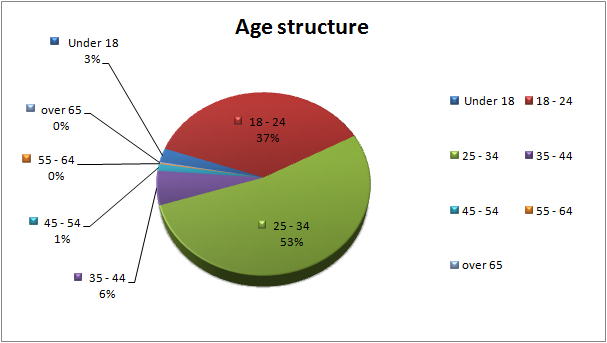
\includegraphics[width=0.5\textwidth]{viral-images/age_structure}
\caption{Age structure of responders.}
\label{fig:age_structure}
\end{figure}

Age structure of the responders is shown on figure \ref{fig:age_structure}.
Most of the responders (90\%) are in the age groups from 25 to 34 and from 18 to 24
years old. Major part of the responders (61\%) are with college degree, 26\% are
with masters degree, and the rest are either high school or Phd.

\begin{figure}
\centering
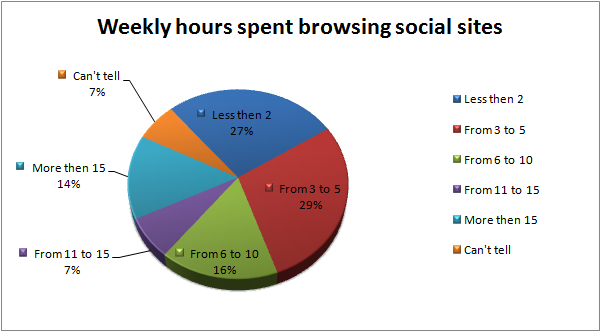
\includegraphics[width=0.5\textwidth]{viral-images/weekly_hours}
\caption{Weekly hours spent browsing social sites.}
\label{fig:weekly_hours}
\end{figure}

Regarding the frequency of browsing social sites, by weekly hours spent
browsing, the results are shown of figure \ref{fig:weekly_hours}. These results
are showing that, 56\% from the responders are spending less than 5 hours
weekly on social sites, and 37\% are spending more then 5 hours weekly. If we
compute the mean value of hours spent weekly, for each age group, then the
result is 6.2 hours spent weekly browsing social sites.

Responses on the question about the location used browsing social sites, none of
the responders answered school as location. Highest percent (85\%) of the
responders are browsing social sites from home, and this confirms the
Hypothesis 2.

\begin{figure}[htb]
\centering
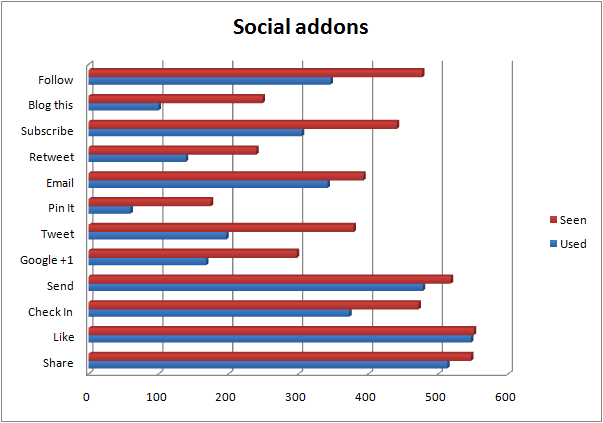
\includegraphics[width=0.5\textwidth]{viral-images/social_addons}
\caption{Social addons.}
\label{fig:social_addons}
\end{figure}

Next questions are about social addons. The first asks if responders have seen
the social addon, and the second one asks if they have used it. Results are
shown on figure \ref{fig:social_addons} and we can see that most used social
addon is \emph{Like}, where the ratio of seen/used is 99\%, and right next to it are
\emph{Share} (94\%), \emph{Send} (92\%) and \emph{Email} (87\%). Least used is
the social addon \emph{Pin it} (34\%), followed by \emph{Blog this} (40\%) and
\emph{Tweet} (53\%).

If we analyze only the results from the responders who visit social networks
every day or multiple times a day, then the ration between seen and used is
increased significantly. These results are confirming hypothesis 3. More time
spent browsing social network, leads to more often usage of social addons.

If we take in to account the gender of responders, men are using more \emph{Subscribe},
\emph{Retweet}, \emph{Tweet} and \emph{Google+1}, and women are using more
\emph{Email}, \emph{Pin it}, \emph{Send}. And if we analyze according to age
groups, the group over 45 mostly use the social addons \emph{Follow},
\emph{Retweet}, while the youngest group mostly use the social addon \emph{Pin
it}. If we take in to account the education level, then the usage of addon \emph{Pin
it} increases with the level of education, and same happens for the social
addons \emph{Tweet} and \emph{Retweet}.

\begin{figure}[htb]
\centering
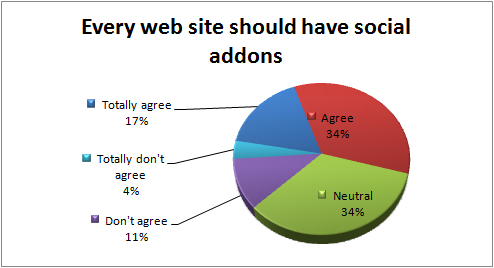
\includegraphics[width=0.5\textwidth]{viral-images/every_web_site}
\caption{Every web site should have social addons.}
\label{fig:every_web_site}
\end{figure}

On figure \ref{fig:every_web_site} is shown what the responders think of the
statement that every web site should have social addons. More than half of them
think are agreeing with the statement, but significant part have neutral
opinion. Roughly 15\% percent of responders do not agree with this statement.
Most of these responders who do not agree are in the age group over 45 years
old.

\begin{figure}[htb]
\centering
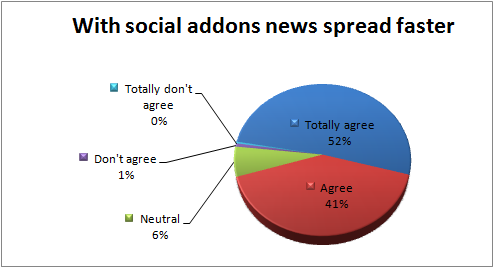
\includegraphics[width=0.5\textwidth]{viral-images/news_spread_faster}
\caption{With social addons news spread faster.}
\label{fig:news_spread_faster}
\end{figure}

Next statement (figure \ref{fig:news_spread_faster}) is about the speed of news
spreading (viral effect). Over 90\% of the responders are agree with this
statement that confirms hypothesis 5. The group over 45 doesn't have a single
member responders that does not agree with this statement. Largest percent of the
responders who do not agree with this statement are in the age groups of up to
25 and from 25 to 45 years old, while those who totally do not agree with this
statement are in the age group up to 25 years old.

\subsection{Results from web site owners}

Second questionnaire has total 24 responders. Answers are from owners of web
sites or blogs in Republic of Macedonia. Regarding the year their site launched,
more then 70\% are from the period from 2010 to 2013. There is a single web site
launched in 1993, 2000, 2003, 2006 and 2007. On the question what is their
target audience, the answers are diverse. There are web sites focused on men,
but also there are sites focused only on women. Some of them answered that their
main target is the younger generation, only supported by audience of parents,
educational workers, city organizations.

\begin{figure}[htb]
\centering
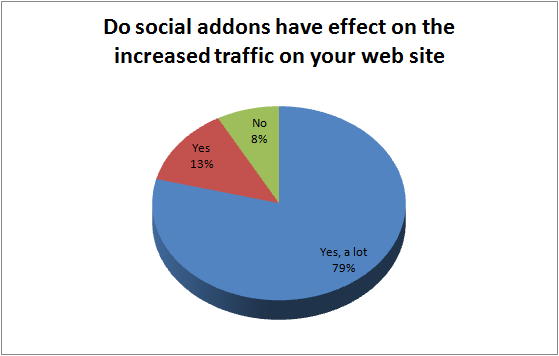
\includegraphics[width=0.5\textwidth]{viral-images/effect}
\caption{Do social addons have effect on the increased traffic on your web
site.}
\label{fig:effect}
\end{figure}

On the question if the content of their site is automatically published to some
social network site, responders answered that they have that implemented only on
the following three social network sites: Facebook (46\%), Twitter (42\%) and
Google+ (8\%).

On the question if social addons have effect on the increased traffic on their
web site, results from answers are shown on figure \ref{fig:effect}. Almost 80\%
of the responders answered that social addons have very big effect on the
increased traffic to their site, 13\% answered that they have small effect, and
only 8\% answered the opposite. These results are confirming hypothesis 5. Those
who answered that social addons do not effect the increased traffic, are using
social addons from the beginning and they spend more than 10 hours weekly in
promotion of their web site on social networks. They have integrated social
addons from Facebook, Twitter and Google+ and the content shared from their web
sites is from diverse categories, mostly once per hour or at least once per day.

Those who answered that social addons have effect on the increased traffic to
their web site, have integrated all the social addons, and they started circa
2012 and most of them are spending from 6 to 10 hours, or more then 15 hours
weekly in promoting their web site on social network sites.

\section{Conclusion}

Results from the survey are confirming most of the presented hypothesis. The
results for the age structure doesn't conclude the first hypothesis, mostly
because the small involvement of the younger age group in the total respondents.
The second hypothesis about the location of the users browsing social sites is
confirmed, and the results are also showing that friendship is not the dominant
motivation for browsing social sites, the fun is stated as most answered choice.

Users spending most hours weekly using social networks, are most often users of
social addons, confirming the third hypothesis. The fourth hypothesis concerned
with the type of content shared is also confirmed, since life style and fun
stories are most shared stories. The fifth and final hypothesis is confirmed
both from users and from owners.
\bibliographystyle{ieeetr}

\bibliography{viral}



\end{document}